\section{Experiments}
\label{sec:exp}
% ~4.5 pages. Report point gains, no significance tests. Standard OVO avg + per-task only (no extra HLD analysis).

\subsection{Setup}
\label{sec:exp-setup}
% Benchmarks: OVO-Bench backward (EPM, ASI, HLD) + real-time (OCR, ACR, ATR, STU, FPD, OJR), 1468 MCQ (631 BT + 837 RT);
%   avg = (BT + RT)/2, Forward not used. StreamingBench real-time, 2500 questions / 500 videos.
% Backbones: Qwen2.5-VL-7B, Qwen3-VL-8B (development), Qwen3-VL-4B (held-out), LLaVA-OneVision-7B (report only).
% Implementation: 1 fps, recent 4 frames, 16 s / 8-frame captions, greedy decoding, scorer = generated letter.
% Baselines: SimpleStream (our rerun, 64.75 vs paper 65.13 on Qwen2.5); D-HSM (public code, same protocol, round 18);
%   ShallowStream (paper values, its own protocol -- marked).
\todo{setup text.}

\subsection{Main Results}
\label{sec:exp-main}
\begin{table*}[t]
  \centering
  \caption{OVO-Bench results (standard avg $=(\mathrm{BT}+\mathrm{RT})/2$). Point gains over SimpleStream in parentheses.
  \todo{per-task RT columns from \texttt{kfs/analyze\_round17.py}; D-HSM rows after round 18.}}
  \label{tab:main-ovo}
  \begin{tabular}{llccccc}
    \toprule
    Backbone & Method & EPM & ASI & HLD & RT & Avg \\
    \midrule
    \multirow{2}{*}{Qwen2.5-VL-7B} & SimpleStream & 53.5 & 61.5 & 40.3 & 77.7 & 64.75 \\
                                   & \method{}    & 53.9 & 64.2 & 73.1 & 77.8 & 70.78 (+6.03) \\
    \midrule
    \multirow{2}{*}{Qwen3-VL-8B}   & SimpleStream & 52.2 & 58.1 & 51.6 & 81.4 & 67.66 \\
                                   & \method{}    & 51.9 & 69.6 & 73.7 & 81.7 & 73.34 (+5.68) \\
    \midrule
    \multirow{2}{*}{Qwen3-VL-4B}   & SimpleStream & 54.6 & 57.4 & 51.6 & 80.3 & 67.42 \\
                                   & \method{}    & 54.2 & 62.8 & 78.0 & 80.2 & 72.60 (+5.18) \\
    \midrule
    \multirow{2}{*}{LLaVA-OV-7B}   & SimpleStream & 55.6 & 54.7 & 20.4 & 74.7 & 59.15 \\
                                   & \method{}    & 58.3 & 57.4 & 31.7 & 74.1 & 61.60 (+2.45) \\
    \bottomrule
  \end{tabular}
\end{table*}
% StreamingBench real-time (no abstention options -> instruction never triggers): ReadPast - SimpleStream =
%   -0.20 / +1.36 / +1.48 / +0.28 (Qwen2.5: 79.76 -> 79.56; Qwen3-8B: 80.28 -> 81.64; LLaVA: 74.64 -> 74.92; 4B: TODO).
\todo{SB table or SB columns; text.}

\subsection{Comparison with Training-Free Methods}
\label{sec:exp-compare}
% D-HSM same protocol (round 18, kfs/analyze_round18_dhsm.py) + D-HSM paper values; ShallowStream paper values
% (Qwen3-8B OVO 69.5 / SB-RT 78.2; LLaVA-OV 62.2 / 75.5), marked "paper value, own protocol".
\todo{after round 18.}

\subsection{Ablation Study}
\label{sec:exp-ablation}
% Table: 2x2 (timeline+gate on/off x conditional instruction on/off) + "instruction on every question" row
% (round 18: Delta cond - always = -0.52 / +1.75 / +1.24 / +0.30). Gate variants (fixed 0.5 vs p_cf; read-all;
% ShallowStream gate). Timeline placement (before vs after recent frames, round 10).
\todo{ablation tables.}

\subsection{Analysis}
\label{sec:exp-analysis}
% (1) Text vs history frames (Qwen3-8B: RT -0.81 vs -4.03 / -5.86; Qwen2.5 similar).
% (2) Timeline content vs foreign timeline (content control): EPM +6.7 / +5.4 own minus foreign.
% (3) Memory reach: gains concentrated within ~90 s of the evidence -> limitation.
% (4) Gate calibration (Fig. 3).
\begin{figure*}[t]
  \centering
  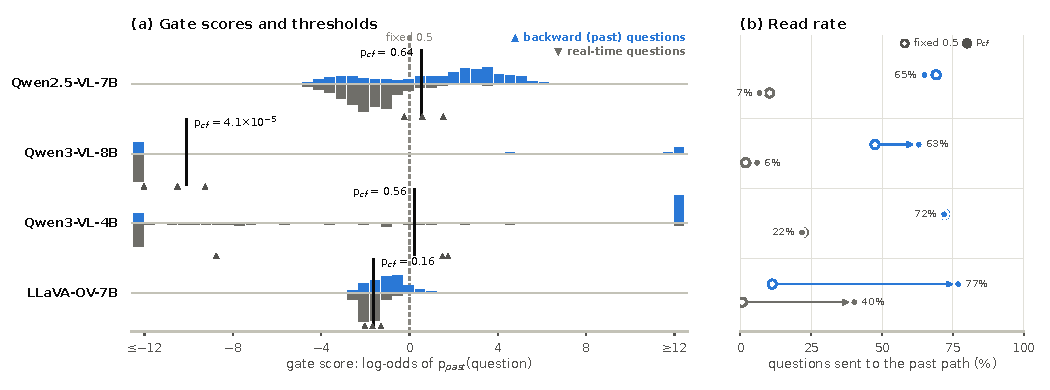
\includegraphics[width=\textwidth]{fig3_calibration.pdf}
  \caption{Content-free calibration of the present/past gate on four backbones. \todo{caption}}
  \label{fig:calib}
\end{figure*}
\todo{analysis text.}

\subsection{Efficiency}
\label{sec:exp-efficiency}
% Round 19 (plan in EXPERIMENTS.md): write cost per stream second (real-time factor), per-question latency
% (gate + answer), peak GPU memory, timeline tokens; SimpleStream / ReadPast / D-HSM on the same GPU, exclusive.
\todo{efficiency table.}

\subsection{Qualitative Results and Failure Cases}
\label{sec:exp-qual}
\todo{2--3 examples: a backward question answered from the timeline; a real-time question kept on frames; a failure
(evidence older than the reach / not written).}
